\section{Durchführung}
\label{sec:Durchführung}
Der Versuch gliedert sich in zwei Teile. Im ersten Teil wird eine Kennlinien der Vakuumdiode aufgenommen und im zweiten Teil wird das Anlaufstromgebiet näher untersucht.

\subsection{Aufnahme der Kennlinien der Hochvakuumdiode}
\label{subsec:D_Kennlinie}
Zuerst wird eine Kennlinienschar der Hochvakuumdiode für fünf verschiedene Stromstärken der Heizstromkreises aufgenommen. Dazu wird der in \autoref{fig:Schaltplan1}
dargestellte Versuchsaufbau verwendet. Der XY-Schreiber wird nicht verwendet, da Spannung und Strom am Spannungsgerät abgelesen werden können.

\begin{figure}
    \centering
    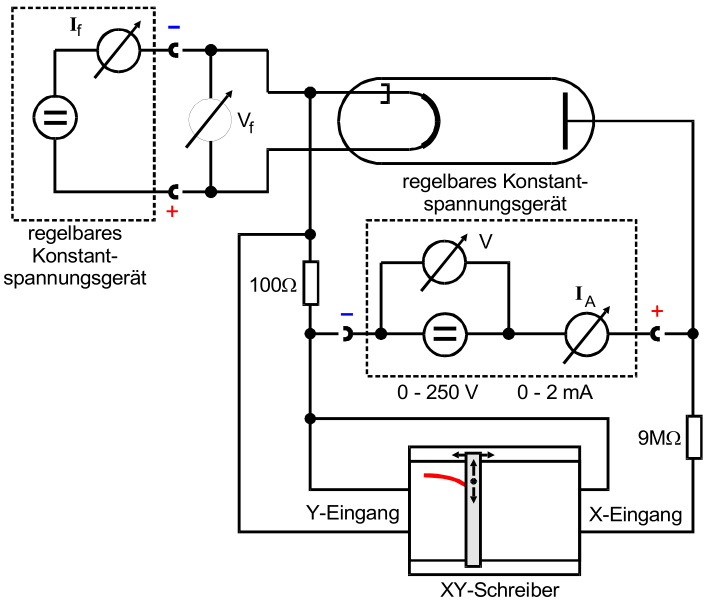
\includegraphics[width = .6\textwidth]{content/Schaltplan1.png}
    \caption{Schaltplan zur Vermessung der Kennlinien der Hochvakuumdiode \cite{v504}.}
    \label{fig:Schaltplan1}
\end{figure}

Am Konstantspannungsgerät des Heizkreises wird ein fester Strom eingestellt. Der Strom sollte dabei den maximalen Diodenstrom (hier: $\qty{2.5}{\ampere}$) nicht übersteigen,
aber auch nicht unter $\qty{1.9}{\ampere}$ gewählt werden. Strom $I_\text{H}$ und zugehörige Heizspannung $U_\text{H}$ werden notiert. Anschließend werden Messwertepaare
der Beschleunigungsspannung $U_\text{B}$ und des Anodenstromes $I_\text{A}$ genommen, bis der Bereich des Sättigungsstromes erreicht ist. Die Schrittweite der Spannung 
sollte an die momentane Änderungsrate der Stromstärke angepasst werden, sodass bei größerer Steigung der Kennlinie mehr Messpunkte zur Verfügung stehen. Das Verfahren wird für
insgesamt 5 Stromstärken des Heizkreises wiederholt, wobei der maximale Heizstrom unbedingt in einer Messreihe erreicht werden sollte.

Aus den so erhaltenen Messdaten lässt sich der Sättigungsstrom zu jeder Kennlinie feststellen, woraus mit der jeweiligen Kathodentemperatur die Austrittsarbeit bestimmt werden kann.
Ebenfalls soll der Exponent der Langmuir-Schottkyschen Raumladungsgleichung \ref{eqn:Raumladung} experimentell ermittelt werden.

\subsection{Untersuchung des Anlaufstromgebietes}
\label{subsec:D_Anlaufstrom}
Zur Vermessung des Anlaufstromgebietes wird die vorherige Schaltung leicht abgeändert. Der neue Schaltplan ist in \autoref{fig:Schaltplan2} dargestellt. 
Da nur sehr geringe Ströme gemessen werden können wird ein sehr empfindliches Amperemeter verwendet.

\begin{figure}
    \centering
    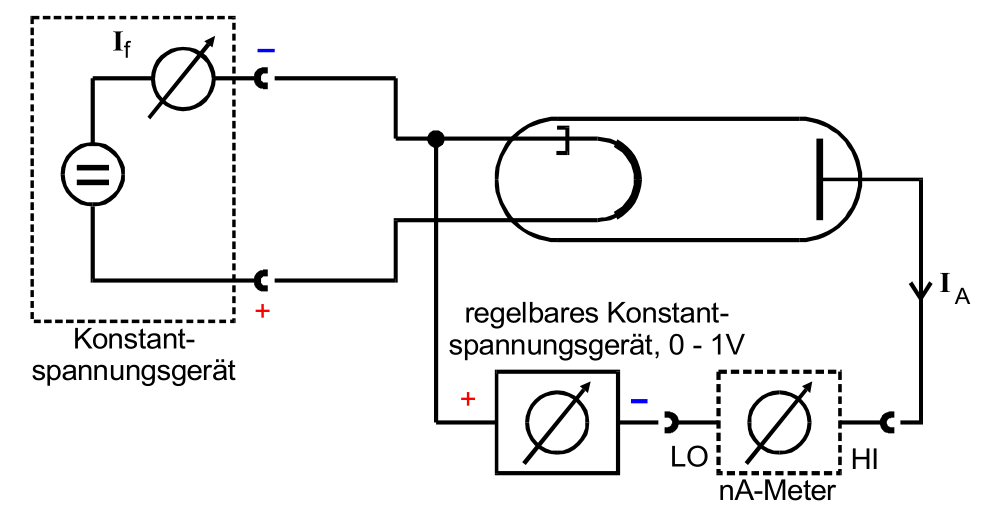
\includegraphics[width = .6\textwidth]{content/Schaltplan2.png}
    \caption{Schaltplan zur Vermessung des Anlaufstromgebietes der Hochvakuumdiode \cite{v504}.}
    \label{fig:Schaltplan2}
\end{figure}

Wie zuvor, wird die maximal mögliche Heizleistung am Spannungsgerät eingestellt. Die Spannung des Gegenfeldes wird in Schritten von $\qty{0.05}{\volt}$ erhöht, während Messwerte
zum Anodenstrom notiert werden. Die Messung wird bei der maximal einstellbaren Spannung von $\qty{1}{\volt}$ beendet.
Da am Innenwiderstand des Amperemeters ein Spannungsabfall hervorgerufen wird, müssen die Werte der Spannung korrigiert werden. 
Dies geschieht nach der Gleichung $U_\text{korr} = U_\text{mess} + I_\text{mess} \cdot R_\text{I}$, wobei $R_\text{I} = \qty{1}{\mega\ohm}$ besagter Innenwiderstand ist.
Aus den Messwerten lässt sich mittels linearer Ausgleichsrechnung die Temperatur $T$ der Kathode bestimmen. 
